\documentclass[tikz]{standalone}
\usepackage{xcolor}
\definecolor{bg}{HTML}{171D2B}
\definecolor{aksen}{HTML}{F7B538}
\definecolor{teks}{HTML}{FFFFFF}
\definecolor{merah}{HTML}{EF4444}
\definecolor{hijau}{HTML}{34D399}
\pagecolor{bg}
\begin{document}
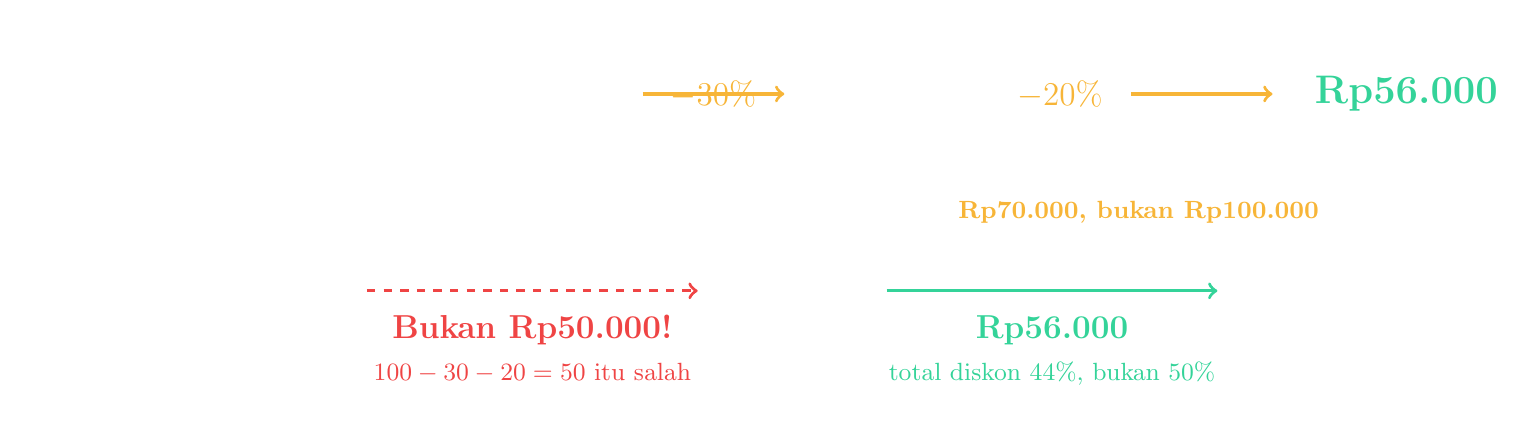
\begin{tikzpicture}[x=1cm,y=1cm]
% price ladder: 100.000 -> -30% -> 70.000 -> -20% -> 56.000
\node[teks, font=\Large\bfseries] at (0,4.4) {Harga Awal: Rp100.000};
\draw[teks, thick] (-0.2,3.9) -- (4.4,3.9);
% first discount
\node[aksen, font=\large\bfseries] at (5.6,3.9) {$-30\%$};
\draw[->, aksen, very thick] (4.7,3.9) -- (6.5,3.9);
\node[teks, font=\Large\bfseries] at (8.2,3.9) {Rp70.000};
% second discount from the NEW base
\node[aksen, font=\large\bfseries] at (10.0,3.9) {$-20\%$};
\draw[->, aksen, very thick] (10.9,3.9) -- (12.7,3.9);
\node[hijau, font=\Large\bfseries] at (14.4,3.9) {Rp56.000};
% explanation band under second step
\node[teks, font=\small, align=center] at (11.0,2.9) {$20\%$ dihitung dari};
\node[aksen, font=\small\bfseries] at (11.0,2.4) {Rp70.000, bukan Rp100.000};
% comparison arrow: wrong expectation
\draw[->, merah, very thick, dashed] (1.2,1.4) -- (5.4,1.4);
\node[merah, font=\large\bfseries] at (3.3,0.9) {Bukan Rp50.000!};
\node[merah, font=\small] at (3.3,0.35) {$100-30-20 = 50$ itu salah};
% final contrast
\draw[->, hijau, very thick] (7.8,1.4) -- (12.0,1.4);
\node[hijau, font=\large\bfseries] at (9.9,0.9) {Rp56.000};
\node[hijau, font=\small] at (9.9,0.35) {total diskon 44\%, bukan 50\%};
\end{tikzpicture}
\end{document}
